\documentclass[journal]{IEEEtran}
\usepackage{url}
\usepackage{listings}
\usepackage[utf8]{inputenc}
\ifCLASSINFOpdf
\else
\fi
\hyphenation{op-tical net-works semi-conduc-tor}
\usepackage{cite}
\usepackage{color}
\usepackage{graphicx}
\usepackage[justification=centering]{caption}

\lstset{
	language=C,                	   % choose the language of the code
	stepnumber=1,                   % the step between two line-numbers.        
  	numbersep=5pt,                  % how far the line-numbers are from the code
  	showspaces=false,               % show spaces adding particular underscores
  	showstringspaces=false,         % underline spaces within strings
  	showtabs=false,                 % show tabs within strings adding particular underscores
  	tabsize=4,                      % sets default tabsize to 2 spaces
  	captionpos=none,                   % sets the caption-position to bottom
  	breaklines=true,                % sets automatic line breaking
  	breakatwhitespace=true,         % sets if automatic breaks should only happen at whitespace
  	keywordstyle=\color{blue},
  	basicstyle=\ttfamily\footnotesize,
  	title=\lstname,                 % show the filename of files included with \lstinputlisting;
}

\begin{document}
\title{Representación del Sistema Solar en OpenGL}

\author{Sebastián Lastra Mena, Amaro Escobar\\ \{sebastian.lastra@usach.cl\}, \{amaro.escobar@usach.cl\}\\Departamento de Matemáticas y Ciencia de la Computación \\ Universidad de Santiago de Chile - Avenida Libertador General Bernardo O'Higgins \#3363 
}

\markboth{TRABAJO DE INVESTIGACIÓN E IMPLEMENTACIÓN - CURSO DE COMPUTACIÓN GRÁFICA, Semestre II - Año 2014}
{Shell \MakeLowercase{\textit{et al.}}}

\maketitle

\begin{abstract}
	En este trabajo se presenta el modelamiento del sistema solar con cinturón de asteroides y la enana roja 	Némesis. Se creó en un ambiente gráfico el cual sufrirá los cambios dependiendo de la elipse que se establezca para la enana roja. Otras implementaciones realizadas en este trabajo fueron la aplicación de texturas en el fondo de la escena utilizando la técnica de SkyBox, el posicionamiento de la ViewPort en la orbita del planeta que se requiera y la implementación de un menu para facilitar la navegación entre las funcionalidades del programa. Fue implementado en OpenGL bajo sistema operativo GNU/Linux.
\end{abstract}

\begin{keywords}
	Sistema Solar, OpenGL, Orbita Elíptica, Nube de Oort, Némesis, SkyBox.
\end{keywords}

\IEEEpeerreviewmaketitle

\section{Introducción}

	La idea principal es llevar a cabo la simulación del Sistema Solar el cual incluye un cinturón de asteroides y la presencia de una enana roja. El sistema que simula el fenómeno espacial se activa presionando un botón, lo cual genera una onda expansiva que desplaza a los asteroides de su cinturón haciendo posible la colisión de estos con los distintos planetas del sistema solar.\\

	Considerando que lo que se presenta en esta versión del informe es una modificación a lo que ya está implementado, resulta importante mencionar que, pese a que se puede pensar que resulta más rápido, fácil e intuitivo implementar los nuevos requerimientos, se tomó gran parte del tiempo para leer, comprender, analizar e interactuar con el programa, con el fin de poder acoplar los nuevos requerimientos y no estropear el resto. Se agregan dos nuevas funcionalidades: la opción de acercarse a las órbitas de los planetas y al llegar a ella comenzar a orbitar en ella, a una velocidad controlada por el usuario. Por otro lado y como se había mencionado anteriormente se aplicó la técnica de SkyBox aplicando una textura de estrellas al fondo de la escena.

\subsection{Objetivo General}
	Generar gráficamente el modelamiento del fenómeno espacial y que se aprecie lo más realista posible. 

\subsection{Objetivos Específicos}
	\begin{itemize}
		\item Aprender a usar las herramientas necesarias de OpenGL para la realización de sombras, iluminación 
		y texturas.
		\item Entender los conceptos fundamentales de la Computación Gráfica y cómo se expresan y/o representan 
		en términos computacionales.
		\item Asociar la teoría aprendida en el curso de Computación Gráfica con la 
		representación práctica en OpenGL.
		\item Lograr un dominio en el lenguaje  de programación y librerías utilizadas.	
	\end{itemize}
	
\section{Definición de la problemática}

En el año 1984, surge una hipótesis astronómica que sustenta de que nuestro Sol forme parte de un sistema binario \cite{RAMuller}. En este sistema, la estrella compañera del sol se llamaría Némesis y cada 26 millones de años desestabiliza la nube de Oort, la cual posee gran cantidad de cometas y estrellas \cite{astronomia}. Esta desestabilización generaría que los cometas que se encuentran en la nube se dirijan hacia el sistema solar causando gran cantidad de colisiones en los planetas. \\

Skybox es una tecnica que permita que una escena se vea más grande y más impresionante, envolviendo al espectador (usuario) con una textura que es posible apreciar en una cámara de 360$^{\circ}$\cite{skybox}. Dicha técnica utiliza imágenes con baja calidad ya que la cantidad de datos que se procesa en cada frame es mucha y si se necesitara una imagen de mayor calidad y/o resolución, es necesaria una tarjeta con procesamiento gráfico independiente para una mejor representación (Además de una optimización en cómo se aplica la textura).\\

Finalmente, resulta necesario trabajar con las transformaciones geométricas correctas que permitan posicionar la viewport en un planeta específico, realizando una trayectoría animada desde un punto $(x_{0}, y_{0}, z_{0})$ hacía un punto $(x_{1}, y_{1}, z_{1})$, considerando que estos orbitan en torno al punto $(0,0,0)$ y sus posiciones varían constantemente.

\subsection{Problemática}
Realizando un desgloce final de las problemáticas de nuestro proyecto, se tiene:\\

\begin{enumerate}
	\item Calcular la trayectoria de los asteroides encontrados en la nube de Oort que impactarán con los planetas.
	\item Encontrar los planetas con los cuales efectivamente harán colisión.
	\item Correcta implementación de la nube de Oort, buscando la mejor representación utilizando OpenGL.
	\item Implementar un menú que permita navegar entre las distintas funcionalidades presentes en el programa.
	\item Aplicar la técnica de SkyBox en la escena.
	\item Realizar la traslación de la ViewPort hacía el planeta deseado utilizando el menú.
\end{enumerate}

\section{Modelo matemático}

\subsection{Ecuación de la elipse}

\begin{figure}[h!]
	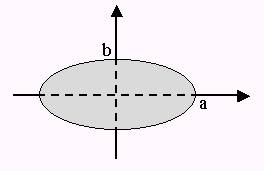
\includegraphics[width=0.25\textwidth, height=0.25\textwidth]{elipse.png}
	\centering
	\caption{Elipse}
\end{figure}

\[ \scalebox{2}{$\frac{x^{2}}{a^{2}} + \frac{y^{2}}{b^{2}}$} \]\\

Donde $a>0$ y $b>0$, las coordenadas de las abscisas. La elipse se encuentra centrada en el origen ($h,k=0$) \cite{enciclopedia}. La ecuación de la elipse modela la ubicación de la nube de Oort y la órbita de los planetas, y la trayectoria de la enana roja Némesis.\\

\[ \scalebox{2}{$ \frac{x\cdot(x-x_{0})}{a^{2}} + \frac{y\cdot(y-y_{0})}{b^{2}}$} \]\\

Luego con la ecuación de la recta tangente a una elipse, se obtiene la dirección a la cual serán lanzadas las estrellas de la nube de Oort, y se observarán las colisiones con los planetas del sistema solar.

\subsection{Matriz de Rotación}

Las rotaciones en dos dimensiones está determinado por la siguiente matriz \cite{foley}:\\
\[ 
	\left[ 
		\begin{array}{cc}
			\cos\theta & -\sin\theta \\
			\sin\theta & \cos\theta
		\end{array}
	\right]
\]

Teniendo esto, es posible generalizar dicha matriz y utilizarla para 3 dimensiones. La diferencia fundamental  radica en que la transformación geométrica de rotación es posible aplicarla sobre $(x,y,z)$, es decir, es posible aplicar la rotación con un ángulo $\theta$ sobre un eje específico. A continuación se presenta cada una de las matrices, indicando sobre qué eje se efectuará la rotación en $\theta$ grados:

Rotación sobre el eje x:\\
\[
	R_{xy}(\theta) = \left[ 
		\begin{array}{cccc}
			1 & 0 & 0 & 0 \\
			0 & \cos\theta & -\sin\theta & 0 \\
			0 & \sin\theta & \cos\theta & 0 \\
			0 & 0 & 0 & 1
		\end{array}
	\right]
\]
Rotación sobre el eje y:\\
\[
	R_{yz}(\theta) = \left[ 
		\begin{array}{cccc}
			\cos\theta & 0 & \sin\theta & 0 \\
			0 & 1 & 0 & 0 \\
			-\sin\theta & 0 & \cos\theta & 0 \\
			0 & 0 & 0 & 1
		\end{array}
	\right]	
\]
Rotación sobre el eje z:\\
\[
	R_{zx}(\theta) = \left[ 
		\begin{array}{cccc}
			\cos\theta & -\sin\theta & 0 & 0 \\
			\sin\theta & \cos\theta & 0 & 0 \\
			0 & 0 & 1 & 0 \\
			0 & 0 & 0 & 1
		\end{array}
	\right]	
\]

Se describe como rotación en los planos $xy$, $yz$ y $zx$, pues resulta más fácil asociar la rotación en 3 dimensiones de esa forma. Por ejemplo, al realizar una rotación $yz$ con $\theta$ grados, el objeto realiza un giro en torno al eje y, pero en el sentido del eje z. Es posible apreciar esto gráficamente con la siguiente imagen:

\begin{figure}[h!]
	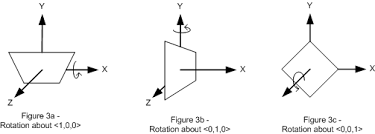
\includegraphics[height=0.15\textwidth]{rotation.png}
	\centering
	\caption{Rotación sobre cada eje.}
\end{figure}

La órbita de los planetas se genera aplicando una rotación sobre el eje $y$ (En el origen, teniendo el solo como referencia) con un ángulo $0^{\circ}\leq\theta\leq360^{\circ}$, el cual aumenta en cada frame de la escena.

\subsection{Matriz de Traslación}

La matriz que describe la traslación de los objetos en la escena es la siguiente:\\

\[ 
	T = \left[ 
			\begin{array}{cccc}
				1 & 0 & 0 & T_{x} \\
				0 & 1 & 0 & T_{y} \\
				0 & 0 & 1 & T_{z} \\
				0 & 0 & 0 & 1 
			\end{array}
		\right] \times 
		\left[ 
			\begin{array}{c}
				v_{x} \\
				v_{y} \\
				v_{z} \\
				v_{w} 
			\end{array}
		\right] = 
		\left(
			\begin{array}{ccc}
				v'_{x} , & v'_{y} , & v'_{z}
			\end{array}
		\right)
\]
\newline

Antes de realizar la rotación de los planetas es necesario posicionarlos en la escena. La traslación de los planetas permite determinar el radio que tendrá la órbita del planeta respecto al sol. Es en torno a esta transformación que se aplica la rotación, por ejemplo, en el primer frame se sitúa el objeto en la posición $(x_{0}, y_{0}, z_{0})$ y se realiza una rotación en $\theta_{0}$ grados en torno al eje $y$, provocando que el objeto se sitúe en la posición $(x_{1}, y_{1}, z_{1})$. Es decir, se aplica un incremento $\Delta$ de la rotación del objeto respecto a su posición original, en cada frame de la escena.

\subsection{Distancia entre dos puntos}

Esta fórmula se utiliza para determinar la distancia entre 2 puntos en un plano en 2D. Si bien el sistema está representado en 3 dimensiones, los planetas se mueven respecto al eje $y$ y la posición de los mismos está determinada sólo por sus coordenadas en el eje $x$ y en el eje $z$. La fórmula traza una línea recta en el plano para determinar la distancia entre los puntos. Las formulas son las siguientes:\\

\[ 
	x_{new} = \frac{\sqrt{X_{final}^{2}+X_{inicial}^{2}}}{100} 
\]
\newline
\[
	z_{new} = \frac{\sqrt{Z_{final}^{2}+Z_{inicial}^{2}}}{100}
\]
\newline

Cabe destacar que el número por el cual se divide cada ecuación (100) es arbitrario y es el que divide la distancia total entre el punto inicial y el punto final, para así generar el efecto de traslación de un objeto desde un punto hacía otro. En este caso el objeto que desplazamos es la viewport. Dicha traslación se realiza hasta que la diferencia entre la posición final y la inicial tenga un valor pequeño, o cercano al punto inicial.

\section{Aproximación utilizada en las simulaciones gráficas}

La formulación del modelo en base al sistema solar y a la teoría de la enana roja respecto al diagrama de Hertzsprung-Russell \cite{russel} es un modelo, debido a que los cálculos realizados son a escala respecto al sistema solar real, es decir, X pixeles son equivalentes a algunos años luz. Los tamaños de los planetas también son a escala y la formulación de las estrellas son pixeles arbitrarios dentro de un rango (cinturón de asteroides).

\section{Implementación computacional}

OpenGl es el principal entorno de desarrollo, para la creación de aplicaciones graficas portátiles e interactivas en  2D y 3D. Desde su introducción en 1992, OpenGl se ha convertido en la Interfaz de Programación de Aplicaciones (API) graficas más usada por la industria, brindando miles de aplicaciones a una gran variedad de plataformas de computación. A su vez, OpenGL fomenta la innovación y velocidad del desarrollo de aplicaciones incorporando una alta variedad de formas de rendering, mapeo de texturas, efectos especiales y otras poderosas funciones de visualización \cite{opengl}.\\

Se utilizo el Entorno de Desarrollo Integrado (IDE) llamado NetBeans, el cual permite detectar rápidamente errores de sintáxis. Permite también iniciar en modo debug, herramienta con la cual es posible realizar un seguimiento del valor de cada variable en cada frame de la aplicación. Además, resulta mucho más fácil el proceso de compilación. La instalación y posterior configuración del proyecto se escapan del ámbito de este informe pero se puede encontrar información respecto a esto en nuestra Wiki del proyecto en GitHub\footnote{Más información en: \url{https://www.github.com/delor34n/nemesis_v2/wiki}}.\\

Como complemento a lo anterior, se utilizó Git para llevar un control exhaustivo de las versiones del código del programa. Además de esto, se hizo uso de los repositorios gratuitos en línea de GitHub\footnote{Proyecto disponible en: "\url{https://www.github.com/delor34n/nemesis_v2}"}, para poder trabajar remotamente, facilitar la integración de los avances de cada integrante del equipo y también para proteger los avances si es que algún computador de alguno de los miembros del equipo falla.\\

Por otro lado, pese a que existe una gran variedad de librerías diferentes a OpenGL, no se utilizaron pues la idea principal de este proyecto es aprender a utilizar al más bajo nivel posible cada uno de los elementos presentes en la computación gráfica (Transformaciones geométricas, primitivas, etc...), cosa que es posible directamente con OpenGL y no con librerías externas que agregan una capa de abstracción en la programación y, por lo tanto, un menor nivel de entendimiento de lo que se realiza. Además, la mayoría de dichas librerías sólo están disponibles para C++.\\

OpenGL trabaja con una pila de matrices, las cuales representan cada objeto que se muestra en la escena. La forma en la que se trabajan dichas matrices es la siguiente:\\

\lstinputlisting{glPushPop.c}  

Como se muestra en ese fragmento de código, se "crea" una nueva matriz dentro de la pila de matrices, se le aplican las texturas y finalmente las transformaciones. Después de esto, se "extrae" la matriz con sus respectivas propiedades y se muestra en la escena según las transformaciones que se hicieron. Es sumamente importante destacar que el orden en que se aplican las transformaciones \textbf{no es aleatorio}. De la misma forma en que se almacenan las matrices en una pila, las transformaciones se aplican de la misma forma, es decir, primero se realiza la traslación (Desde el origen hacía el punto $(x,y,z)$) para posteriormente realizar la rotación sobre el eje deseado. Es vital mantener dicho orden de ejecución, ya que sintáxticamente el programa estará correcto, porque si se realizan las transformaciones al revez, primero tendremos una rotación del objeto sobre sí mismo (Respecto al eje deseado) y luego se aplicará la traslación, provocando que el objeto quede en el mismo lugar siempre.

Las transformaciones geométricas en OpenGL están implementadas y es posible utilizarla con las siguientes funciones:

\subsection{glRotate}

Función que realiza la rotación de un objeto, en torno a un eje a elección, utilizando transformaciones geométricas\cite{glrotate}. El prototipo de dicha funcion es el siguiente:

\lstinputlisting{glRotate.c} 

Donde $angle$ es el ángulo que se le aplicará y $(x,y,z)$ es sobre el eje que se aplicará la rotación \footnote{Se determina con un 1 sobre el eje en que se realiza la rotación, el resto va con ceros. Se utilizan dichos valores pues están normalizados, y si se utiliza cualquier otro valor, OpenGL internamente los normaliza}. Resulta importante destacar que, tanto el ángulo de rotación como las coordenadas, pueden ser variables de tipo \textbf{float} y \textbf{double}.\\

Dicha función no utiliza la misma matriz para realizar la transformación geométrica que se menciona anteriormente, en cambio utiliza la siguiente:\\

\[
	\left( 
		\begin{array}{cccc}
			x^{2}(1-c)+c & xy(1-c)-zs & xz(1-c)+ys & 0 \\
			yx(1-c)+zs & y^{2}(1-c)+c & yz(1-c)-xs & 0 \\
			xz(1-c)-ys & yz(1-c)+xs & z^{2}(1-c)+c & 0 \\
			0 & 0 & 0 & 1
		\end{array}
	\right)
\]\\

Donde: $c = \cos\theta$ y $s=\sin\theta$.

\subsection{glTranslate}

Función que realiza la traslación de un objeto, la cuál está determinada por un vector que se proyecta desde el origen hasta la coordenada $(x,y,z)$ deseada\cite{gltranslate}. El prototipo de la función es el siguiente:

\lstinputlisting{glTranslate.c} 

Resulta trivial darse cuenta que $(x,y,z)$ es hacía dónde se quiere mover el objeto. Esta función utiliza la misma matriz descrita en la sección anterior.

\subsection{gluLookAt}

Función que se utiliza principalmente para fijar el punto desde dónde se observará la escena \cite{glulookat}. El prototipo de esta función es el siguiente:

\lstinputlisting{gluLookAt.c}

Donde:

\begin{itemize}
	\item \textbf{\textit{eyeX, eyeY, eyeZ}}: Coordenada $(x,y,z)$ en la que se posicionará el punto de vista.
	\item \textbf{\textit{centerX, centerY, centerZ}}: Coordenada $(x,y,z)$ que especifíca el punto de referencia hacía el cual se posicionará el punto de vista.
	\item \textbf{\textit{upX, upY, upZ}}: Vector que determina la dirección.
\end{itemize}
                
Para un mejor entendimieno del cómo trabaja la función gluLookAt, debemos entender el punto de vista como un objeto más en la escena, casi cómo una cámara. Al verlo de esta manera, podemos concluir que ésta tiene asociada una matriz (como cualquier otro objeto de la escena), para poder situarla dentro de la escena y así se pueda usar su matriz para modificar la orientación y/o ubicación del punto de vista en la escena. Esto quiere decir que podemos aplicar transformaciones geométricas (glRotate y glTranslate) también a nuestra "cámara" para situarla donde se requiera. Esto se puede representar con lo siguiente:

\[
	M = T * R
\]

Siendo $M$: matriz de la viewport, $T$: matriz de traslación y $R$: matriz de rotación. Se puede apreciar mucho didácticamente con la siguiente imagen:

\begin{figure}[h!]
	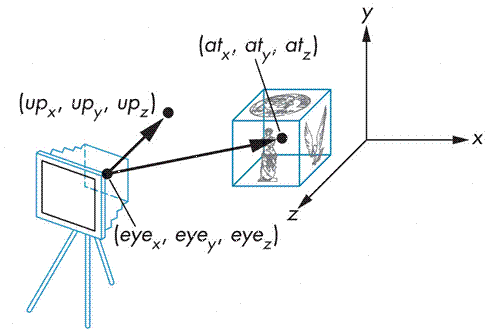
\includegraphics[width=0.4\textwidth, height=0.25\textwidth]{viewport.png}
	\centering
	\caption{Representación gráfica del punto de vista en la escena, utilizando gluLookAt.}
\end{figure}

\subsection{walkFromTo}

Esta función permite acerca la viewport (con ayuda de la función gluLookAt) hacía los planetas. La función es la siguiente:

\lstinputlisting{walkFromTo.c}

Dicha función recibe como parámetros el punto inicial y el punto al que se quiere llegar. Los primeros 2 parámetros corresponden a la posición donde está la cámara en determinado momento, y los últimos 2 parámetros corresponden hacia dónde quiero desplazarme. Se utilizó un divisor de 100 en la fórmula para lograr que el movimiento se vea más fluido, pero se puede cambiar a discreción. Para generar una condición de stop para que no se acerque infinitamente al punto que queremos ir (ya que si no se utiliza esta condición, las distancias serán cada vez más pequeñas hasta el punto en que será innecesario seguir dividiendo la distancia).

\subsection{getOrbitStartPoint}

Esta función recibe como parámetro el ángulo de rotación del planeta, el vector en dónde se almacenarán las coordenadas luego de la rotación, y la posición en $(x,y,z)$ respecto al origen desde la cuál se comienza a realizar la órbita. Esta función utiliza la matriz de rotación (vista en la sección anterior) respecto al eje $y$. La función es la siguiente:

\lstinputlisting{getOrbitStartPoint.c}

Esta función realiza el producto de la multiplicación de la matriz de rotación respecto al eje $y$ por el vector de la posición inicial (correspondiente al planeta).

\subsection{Keyboard}

Dentro de las funcionalidades del programa, se encuentra la posibilidad de aumentar o disminuir la velocidad con la que se realiza el seguimiento del planeta. Dicho control funciona mediante la siguiente función:

\lstinputlisting{keyboard.c}

Cada planeta orbita según un ángulo $\theta$. Dicho ángulo se obtiene la siguiente fórmula:\\

\[
	angulo = (( dia / 365)*360)/(factor*(speed));
\]\\

Donde $dia$ es una variable que aumenta en una unidad en cada frame. La operación que se realiza es la división de un día en 365 (1 Año, es decir, tiempo que tarda la tierra en dar una vuelta completa al sol) multiplicado por 360 (Representando los $360^{\circ}$ de una circunferencia), dividido por un $factor$ (El cual correspondiente a cada planeta). A este último factor se le aplica una multiplicación ($speed$), lo cual permite que el resultado de la división, es decir, el ángulo de rotación que se le aplica al objeto respecto al eje $y$, sea más pequeño (La velocidad disminuya) o sea más grande (La velocidad aumente). Las teclas que permiten controlar esto son las teclas \textbf{'j'} y \textbf{'k'}.

\subsection{loadSkyBox}

Antiguamente, la mayoría de los video juegos utilizaban esta técnica, ejemplo de esto es Doom II. La escena de dicho juego se sitúa en el interior de un cubo gigante, dando la impresión de que Keen (Personaje que maneja el usuario) se encuentra en la tierra:

\begin{figure}[h!]
	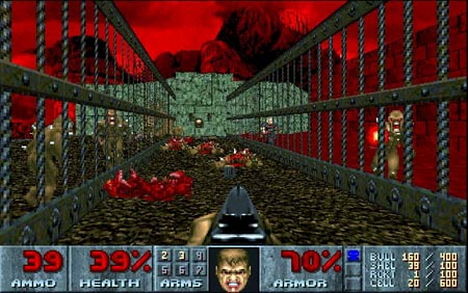
\includegraphics[width=0.4\textwidth, height=0.25\textwidth]{doom2.jpg}
	\centering
	\caption{Doom II: Hell on Earth.}
\end{figure}

La idea detrás de la técnica Skybox, es renderizar un cubo gigante con una textura particular, posicionando la escena y la viewport en el centro\cite{skybox2}.\\

Existen dos tipos de Skybox: basado en texturas (mapeo de la textura en un cubo) y otro basado en geometría (Situar la viewport en un punto inaccesible al usuario y desde allí proyectar el fondo). Para efectos de este proyecto se utilizará el primero.

Como se decía anteriormente, se aplica un tipo especial de textura en el cubo. Esta textura se crea de forma que cada cara del cubo posea la textura que le corresponde y que al interior del cubo las esquinas estén perfectamente alineadas, para crear la sensación de una textura continua. La textura que se aplicó es la siguiente:

\begin{figure}[h!]
	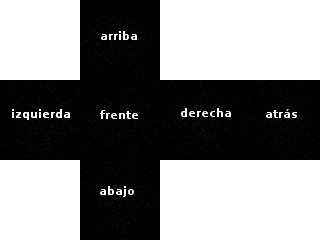
\includegraphics[width=0.4\textwidth, height=0.25\textwidth]{skybox.png}
	\centering
	\caption{Textura utilizada para realizar el SkyBox en la escena.}
\end{figure}

El procedimiento que se realiza, es cortar cada segmento en una imagen diferente y, en el interior del programa, cada una se trabaja como textura independiente. Posterior a eso, se crea un cubo gigante y se le aplica la textura:

\begin{figure}[h!]
	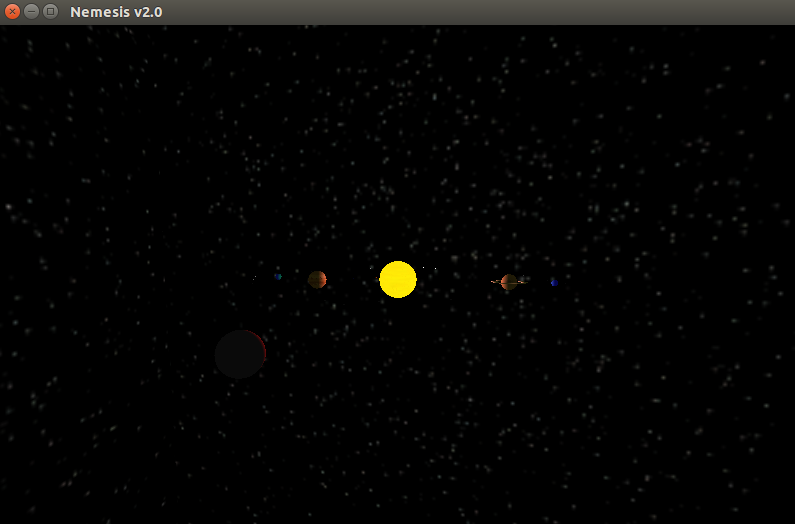
\includegraphics[width=0.4\textwidth, height=0.25\textwidth]{skybox_example.png}
	\centering
	\caption{Ejemplo de la ejecución del programa.}
\end{figure}

Cabe destacar que el formato de imagen utilizado fue el mismo que se utiliza para cargar las texturas de los planetas (TGA) y esto fue porque es la forma más óptima de ahorrar los costos de renderizando, utilizando un formato de imagen que es de fácil lectura y de una calidad menor.

\subsection{Menu de opciones}

Básicamente, se incorporaron las funcionalidades existentes y se agregaron las nuevas:

\begin{enumerate}
	\item \textbf{Go Nemesis!}: Inicia la animación de Nemesis.
	\item \textbf{Iniciar movimiento}: Inicia la animación de los planetas orbitando.
	\item \textbf{Detener movimiento}: Detiene la animación de los planetas orbitando.
	\item \textbf{Ir a}: Uno de los requerimientos fue acercarse a cada planeta y girar en la órbita del mismo.  Para esto está el submenú "Ir a", donde seleccionando cada planeta la viewport se desplaza inmediatamente a la órbita de este, acercándose desde la posición donde está en el momento en el que se selecciona la opción, hasta la órbita del planeta requerida. Al llegar a la órbita del planeta, la viewport comenzará a rotar en torno al sol.
\end{enumerate}

A continuación una imágen del menú:

\begin{figure}[h!]
	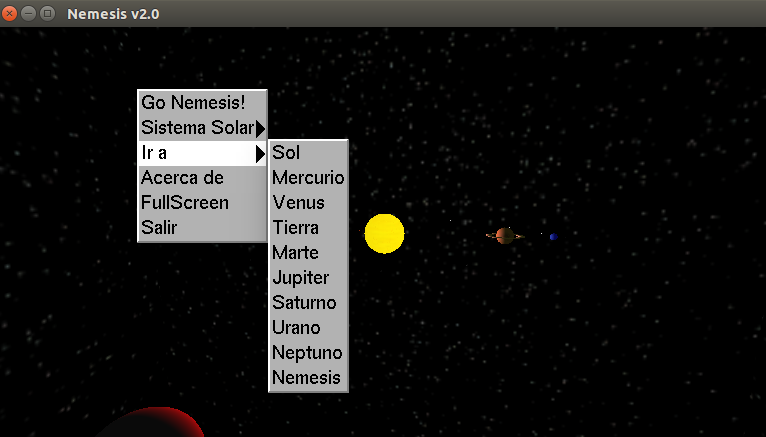
\includegraphics[width=0.4\textwidth, height=0.25\textwidth]{menu.png}
	\centering
	\caption{Menu.}
\end{figure}

\section{Análisis de resultados}

\subsection{Validación de resultados}

 El trabajo es realizado es en base a un proyecto anterior del ramo de Computación Gráfica, llamado Sistema Solar \cite{anterior}. Este proyecto ha sido optimizado en líneas de código y utilizado para nuestro proyecto de fin de semestre. El hecho de que la nube de Oort no se pueda apreciar desde nuestro planeta, y de que la estrella Némesis sea una hipótesis astronómica, deja a la “realidad” un poco de lado. Se corresponde sí a las hipótesis científicas, a las distancias normalizadas de los planetas y sus velocidades de rotación.

\subsection{Rendimiento gráfico de la aplicación}

La aplicación realizada quedo implementada de tal manera que su visualización es, si no rápida, realista a un nivel a escala del fenómeno real es decir, podría verse tanto en un pc especializado (poseedor de una buena tarjeta de video) o en un pc común  corriente. La aplicación es óptima respecto al trabajo que tomamos de base, ya que se redujeron las líneas de código, sin perder la efectividad y el fondo de la aplicación destacando los 2 puntos anteriores. El rendimiento gráfico de la aplicación es prudente(por la sencillez), rápido(por como se aprecia) y optimo(por cómo se realiza).

\subsection{Resultados y Problemáticas}

Como problema de implementación, tenemos un equipo al cual se le instaló el SO Linux Ubuntu, el cual no posee aceleración gráfica, por lo que el proyecto no alcanza su máximo corriendo en esa máquina. No se alcanza a distinguir los movimientos de los planetas y pierde valores al momento de compilar. Por ende, la programación en ese equipo se ha vuelto truncado por problemas que escapan a cualquier tipo de solución que podamos dar. 

La mayor problemática que se presentó fue el determinar la posición exacta de cada planeta en cada frame y esto se debe a que la función $glRotate$ de OpenGL, utiliza otra matriz para realizar la transformación. Pese a esto, se realizó una aproximación utilizando la matriz de rotación vista en clases, permitiendo realizar el seguimiento del planeta en su orbita. Esto se podría haber evitado si la implementación de la órbita de cada planeta se hubiese hecho sabiendo a priori las posiciones de cada planeta en cada frame.

\section{Experimentos}

En la imagen se puede apreciar la estrella Némesis (situada en la esquina inferior derecha) sin haber tocado los asteroides de la nube de Oort:

\begin{figure}[h!]
	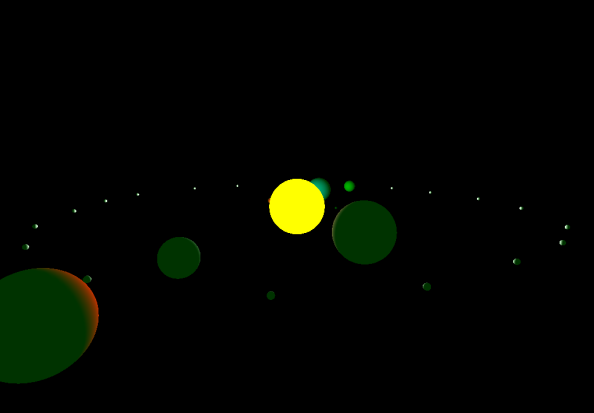
\includegraphics[width=0.4\textwidth, height=0.25\textwidth]{imagen_fea.png}
	\centering
	\caption{Los asteroides todavía tienen su orbita normal.}
\end{figure}

Posteriormente en la siguiente imagen se puede ver como son desplazados los asteroides al perder su órbita normal y ser atraídos por el sol:

\begin{figure}[h!]
	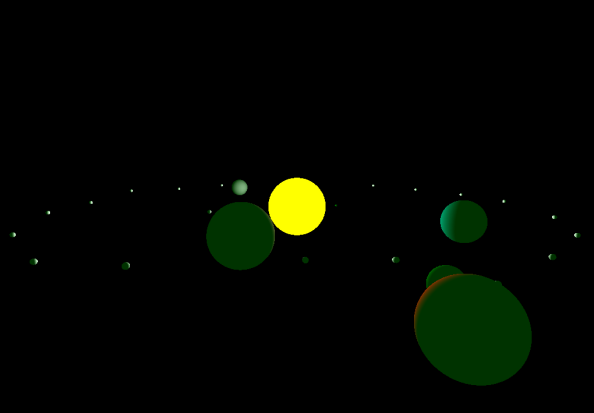
\includegraphics[width=0.4\textwidth, height=0.25\textwidth]{imagen_fea2.png}
	\centering
	\caption{La orbita de los asteroides ha sido cambiada gracias al
movimiento de la estrella Némesis.}
\end{figure}

El resto de los experimentos es posible apreciarlos en los videos adjuntos a este informe.

\section{Conclusiones}

La realización de este modelamiento fue costosa y ardua, ya que no había conocimiento de cómo plantearnos el problema, tal vez bosquejos o ideas que cualquier persona podría tener, pero no como analistas. Luego de algunas clases y laboratorios empezamos a entender lo que nos pedían y como poder realizar el modelamiento. Después de mucha investigación, comprensión de códigos antiguos, adquisición de conocimientos sobre el lenguaje de programación utilizado y el trabajo de unas funciones, se pudo llevar a cabo el modelamiento final. Nos sentimos orgullosos de haber sido capaces de realizar un buen modelamiento de un fenómeno natural tan sorprendente. De aquí en adelante esperamos que este trabajo pueda ser reutilizado como base para proyectos mas grandes por alumnos que tendrán este ramo más adelante o bien ser capaz de optimizarlo y lograr difundirlo para algún uso particular de buena manera.

\bibliographystyle{IEEEtran}
\bibliography{bibi}

\end{document}